% !TEX root = ../main.tex

% Local Variables:
% TeX-master: "../main"
% End:
% chktex-file 26

%%%%%%%%%%%%%%%%%%%%%%%%%%%%%%% Header %%%%%%%%%%%%%%%%%%%%%%%%%%%%%%%%%%%%%%%%%%%%
\begin{minipage}[l]{0.42\textwidth}
    
\includegraphics[width=1\textwidth]{img/logo-UNAMBA.png}
\end{minipage}
\hfill
\begin{minipage}[c]{0.5\textwidth}
    \begin{flushright}
	\large{\textbf{Unidad \#2}}\\
	\large{Lectures on Física III}\\
	\large{24 de Julio del 2025. Haquira, Apurimac}\\
        % \large{\textbf{Student:} Huallpa Aimituma Josué David}
    \end{flushright}
\end{minipage}
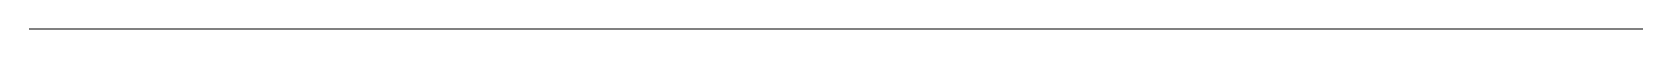
\begin{tikzpicture}
    \draw[gray,thick] (-6.5,0)--(14,0);
\end{tikzpicture}


 %%%%%%%%%%%%%%%%%%%%%%%% INICIO DEL CONTENIDO EN DOS COLUMNAS %%%%%%%%%%%%%%%%%%%%%
  
 \begin{multicols}{2}
   \begin{center}
         \LARGE{\textbf{Capítulo V: Circuitos RC}}\\	
         \vspace{0.2cm}
         % \Large {Lecturers Esteban Chalbaud \& Daniel Galviz} \\
         % \large{Teaching Assistant: Mauricio Gamonal \& Irvin Martínez}\\
         % \large{PhysicsLatam.com}\\
         % \vspace{0.2cm}
         \large{28 Agosto 2025, 6:59 am (GMT-4)}\\
         % \vspace{0.2cm}
         \large{— Evaluación Parcial 3 —}
     \end{center}
    %%%%%%%%%%%%%%%%%%%%%%%%%%%%excercise%%%%%%%%%%%%%%%%%%%%%%%%%%%%%%%%%%%%%%%%
    \begin{excercise}[][][]{ex:k28}{(\textbf{4 pts})
        \textbf{(Preguntas teóricas)}
        \begin{itemize}
            \item[a)] Es cierto que la relación 
                \begin{equation*}
                                    R=\frac{V}{I}
                                \end{equation*}
                                es una expresión de la ley de Ohm, o también debe satisfacer alguna otra condición? Grafíque esta relacón. 
                            \item[b)] Dos conductores tienen la misma resistencia y la misma longitud, pero uno de ellos tiene el doble de sección transversal que el otro. ¿Cómo está relacionadas las conductividades de los dos?
                            \item[c)] Defina que es la potencia disipada por una resistencia, a partir de la ley de Ohm, encuentre las tres ecuaciones en función del voltaje y la corriente que són utiles para calcularla.
                            \item[d)] Delimite cualitativamente cuales son los límites aproximados de voltaje y corriente eléctrica al que un ser humano puede estar expuesto con seguridad. 10A con 50V es un rango seguro? comente del mismo modo para 
                                \begin{itemize}
                                    \item 1A, 100V
                                    \item 100A, 1V
                                    \item 1A, 30V
                                    \item 0.002 A, 100 000 A
                                \end{itemize}
        \end{itemize}
         }
    \end{excercise}
        \begin{excercise}[][][]{ex:k28}{(\textbf{4 pts})
        \textbf{(Circuitos RC)}
            A partir de un circuito RC simple, determinar la expresión del corriente eleéctrica y el voltaje que circula por el circuito como función del tiempo.
             \vspace{8cm}
         }
    \end{excercise}
   
    %%%%%%%%%%%%%%%%%%%%%%%%%%%%excercise%%%%%%%%%%%%%%%%%%%%%%%%%%%%%%%%%%%%%%%%
        %%%%%%%%%%%%%%%%%%%%%%%%%%%%excercise%%%%%%%%%%%%%%%%%%%%%%%%%%%%%%%%%%%%%%%%
    \begin{excercise}[][][]{ex:19}{(\textbf{12 pts})
       Para las Fig. Calcular la corriente que circula por cada resistencia, la diferencia de potencial y la potencia disipada si cada resistor es de 200 $\Omega$, $\varepsilon_1=9V$,$\varepsilon_2=5V$ y $\varepsilon_3=7V$ 
        \begin{figure}[H]
            \centering
            \includegraphics[width=0.6\linewidth]{img/01_physics-i/03_statics/1.1.png}
        \end{figure}
         \begin{figure}[H]
            \centering
            \includegraphics[width=0.6\linewidth]{img/01_physics-i/03_statics/2.2.png}
        \end{figure} 
    } 
          \begin{figure}[H]
            \centering
            \includegraphics[width=0.6\linewidth]{img/01_physics-i/03_statics/3.3.png}
        \end{figure}
         \begin{figure}[H]
            \centering
            \includegraphics[width=0.7\linewidth]{img/01_physics-i/03_statics/4.4.png}
        \end{figure}
    \end{excercise}
\end{multicols}
